
\documentclass[addpoints,12pt]{exam}
\usepackage{amssymb,amsmath,amsthm,graphicx}
\usepackage{tikz}
\usepackage{listings}
\usepackage{courier}
\usepackage{graphics}
\usepackage{scrextend}
\usepackage{adjustbox}

\lstset{frame=l,xleftmargin=\fboxsep,xrightmargin=-\fboxsep,colframe=gray}
\lstset{basicstyle=\ttfamily\footnotesize,breaklines=true}


\newcommand{\code}[1]{{\texttt{#1}}}
\newcommand{\mcode}[1]{{\text{\texttt{#1}}}}

\linespread{1.2}
\usepackage{color}
\definecolor{gray}{rgb}{0.3,0.3,0.3}



\pagestyle{headandfoot}
\runningheadrule
\firstpageheader{Math 9}{\,}{Practice Final}
\runningheader{Math 9}
              {\,}
              {Practice Final, Page \thepage\ of \numpages}
\firstpagefooter{}{}{}
\runningfooter{}{}{}
\newtheorem{theorem}{Theorem}
\newtheorem{definition}{Definition}
\newtheorem{expectation}{Expectation}

\newcommand{\RR}{\mathbb{R}}

\begin{document}
\begin{center}
\fbox{\fbox{\parbox{5.5in}{\centering
{\tt Directions:} The exam is 120 minutes long. Please read each question carefully. 
\vspace{10pt}

When asked to write code, you should write working Python code that has correct syntax. You should explain in 1-2 sentences what the idea for your solution is or write next to your code what it is doing. This will increase your chances of getting full/partial credit. 

Use the backs of the pages if needed.
}}}
\end{center}


\vspace{0.2in}

\makebox[\textwidth]{Last Name:\enspace\hrulefill}

\vspace{0.2in}

\makebox[\textwidth]{First Name:\enspace\hrulefill}

\vspace{0.2in}

\makebox[\textwidth]{Student ID \#:\enspace\hrulefill}

\vspace{0.2in}

\vspace{1in}

\gradetable

\newpage

\begin{questions}

\question[20]
Write down the output of the following programs.

\begin{enumerate}
\item 
\begin{lstlisting}[language=python]
x = 1
s = 0
for i in range(8):
    s += x
    x += 1
print(s)
\end{lstlisting}
\vfill


\item 
\begin{lstlisting}[language=python]
def f(n):
    if n > 0:
        return n * g(n)
    return 1

def g(n):
    return f(n // 2)

print(f(6))
\end{lstlisting}
\vfill


\item 
\begin{lstlisting}[language=python]
from functools import reduce
x = reduce(lambda a,d: 2*a+d, [1,0,0,0,0,1,0,1])
print(x)
\end{lstlisting}
\vfill

\item 
\begin{lstlisting}[language=python]
def f(xs):
    if xs == []:
        return 0
    return xs[0] + f(xs[1:])

f([1,2,3,4,5])
\end{lstlisting}
\vfill


\end{enumerate}

\newpage
\question[20] Produce the following lists without using for or while loops. 
\begin{enumerate}
  \item \code{[0, 1, 3, 7, 15, 31, 63, 127, 255, 511]}
    \vfill
  \item \code{[1, 2, 4, 5, 7, 8, 10, 11, 13, 14, 16, 17, 19]}
    \vfill
  \item \code{[-1, 2, -3, 4, -5, 6, -7, 8, -9, 10, -11, 12, -13, 14]}
    \vfill
\end{enumerate}


\newpage
\question[20] Write code that will produce the following graphs (or something that looks like it; use \code{plt.plot(X, Y)} and \code{plt.scatter(X, Y)}).
\begin{enumerate}
\item
\adjustbox{valign=t}{
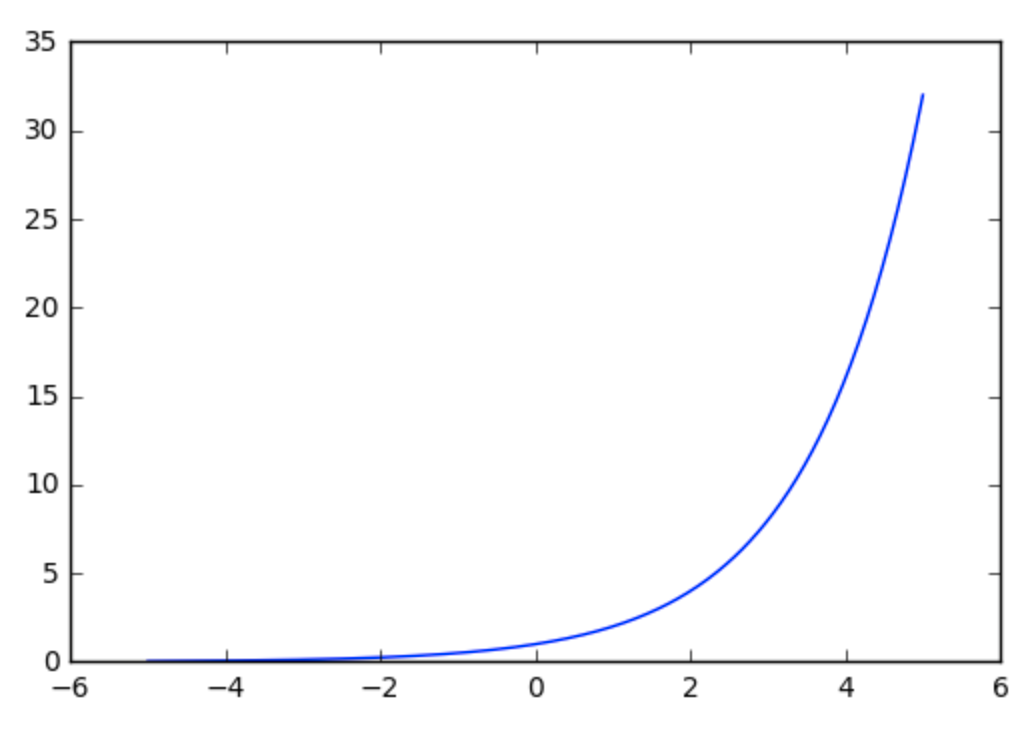
\includegraphics[valign=t, width=3.1in]{graph_exp.png}
}
\vfill
\item 
\adjustbox{valign=t}{
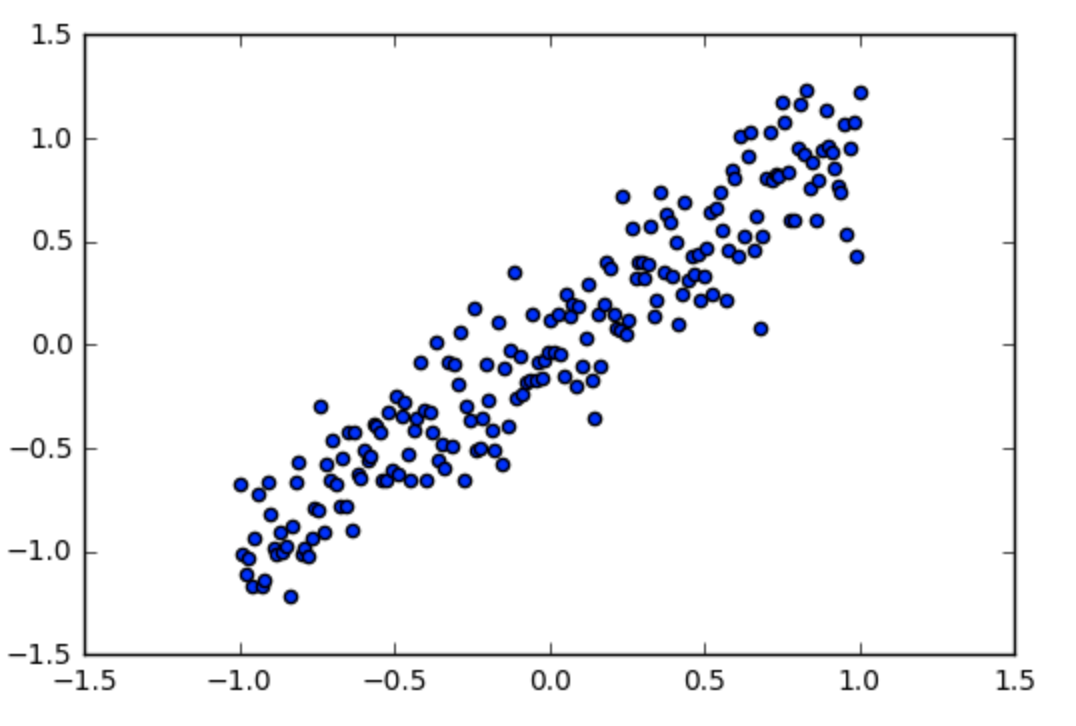
\includegraphics[valign=t, width=3.2in]{graph_noise_lin.png}
}
\vfill
\end{enumerate}


\newpage
\question[20] Complete the code below to implement the function \code{chessboard(n)} that will return a numpy array with 1's and 0's arranged in a chessboard pattern. You can assume \code{n} is odd. 
Examples:
\begin{lstlisting}[language=python]
In:   chessboard(3)
Out:  array([[0, 1, 0],
             [1, 0, 1],
             [0, 1, 0]])

In:   chessboard(5)
Out   array([[0, 1, 0, 1, 0],
             [1, 0, 1, 0, 1],
             [0, 1, 0, 1, 0],
             [1, 0, 1, 0, 1],
             [0, 1, 0, 1, 0]])
\end{lstlisting}

\begin{lstlisting}[language=python]
def chessboard(n):
    X = 
    return 
\end{lstlisting}

\vfill

Complete the code below to implement the function \code{chessgonewrong(n)}, which produces a chess-board with the middle $3\times 3$ square having $-1$'s instead of $1$s.
\begin{lstlisting}[language=python]
In:   chessgonewrong(7) 
Out:  array([[ 0,  1,  0,  1,  0,  1,  0],
             [ 1,  0,  1,  0,  1,  0,  1],
             [ 0,  1,  0, -1,  0,  1,  0],
             [ 1,  0, -1,  0, -1,  0,  1],
             [ 0,  1,  0, -1,  0,  1,  0],
             [ 1,  0,  1,  0,  1,  0,  1],
             [ 0,  1,  0,  1,  0,  1,  0]])
\end{lstlisting}

\begin{lstlisting}[language=python]
def chessgonewrong(n):
    X = chessboard(n)

    return X
\end{lstlisting}
\vfill


\newpage
\question[20] Implement a function \code{divisors(n)} that returns all positive integer divisors of an integer \code{n} as a list. (returns not prints)

\newpage
\question[20] A palindrome is a word that is the same when reversed, e.g. ``amanaplanacanalpanama''. Write a function \code{ispalin(s)} that will return \code{True} if a string \code{s} is a palindrome and \code{False} otherwise. (remark: you can work with \code{s} as if it were a list). 



\newpage
\question[20] Recall the \code{Polynomial} class from the homework that stores a polynomial as a list of its coefficients. Implement the \code{\_\_add\_\_(self, other)} function that returns a new polynomial which represents the sum of the polynomials \code{self} and \code{other}.  

\begin{lstlisting}[language=python]
class Polynomial():
    def __init__(self, xs):
        self.coeffs = xs
   
    # returns a string representation of the polynomial
    def __repr__(self):
        if self.coeffs == []:
            return "0"
        c = ""
        for i, x in enumerate(self.coeffs):
            c += str(x) + "x" + "^" + str(i) + " + "
        return c[:-3]
    
    def __add__(self, other):
\end{lstlisting}

\newpage
\question[20] Write code that will find the minimum of the function $f(x,y) = x^4 + y^2 + 2x + 4y + 1$ using gradient descent. (Start the descent from $(x,y) = (5,5)$ and use the learning rate of $\eta = 0.01$). Your code should print the minimum value it finds. 


\end{questions}
\end{document}
